\documentclass[tikz]{standalone}
\begin{document}

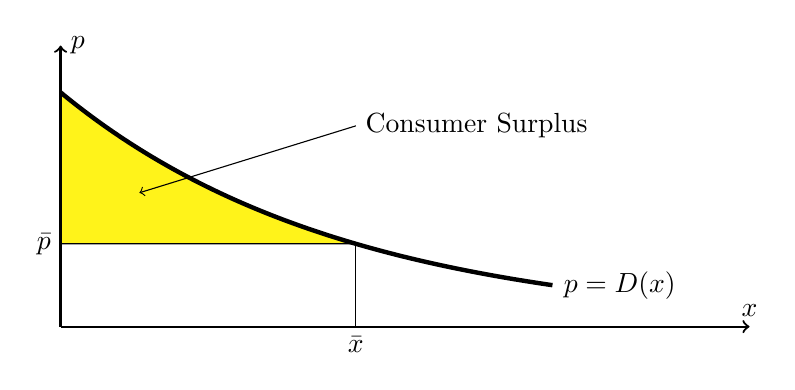
\begin{tikzpicture}[xscale=2.5,yscale=0.85]

  % shade region
  \draw[fill=yellow!90] plot[smooth, samples=10, domain=0:1.5] (\x,3.5/2^\x) |- (0,1.237) -- cycle;
    
  % draw axes 
  \draw[thick,->] (0,0) -- (3.5,0) node[above] {$x$};
  \draw[thick,->] (0,0) -- (0,4.2) node[right] {$p$};
    
  % draw curve
  \draw[ultra thick,domain=0:2.5,samples = 100, smooth,variable=\x,black] plot ({\x},{3.5/2^\x})node[right] {$p=D(x)$};

  \draw (1.5,1.237) -- (1.5,0) node[below] {$\bar{x}$};
  \draw (1.5,1.237) -- (0,1.237) node[left] {$\bar{p}$};
  \draw[<-] (0.4,2) -- (1.5,3) node[right] {Consumer Surplus};
\end{tikzpicture}
\end{document} 
